\documentclass{article} % For LaTeX2e
\usepackage{nips13submit_e,times}
\usepackage{hyperref}
\usepackage{url}
%\documentstyle[nips13submit_09,times,art10]{article} % For LaTeX 2.09

\usepackage{tikz}
\usetikzlibrary{shapes.geometric, arrows}
\usetikzlibrary{positioning,arrows}

\tikzstyle{process} = [rectangle, rounded corners, minimum height=1cm, text centered, text width=2cm, draw=black, font=\scriptsize]
\tikzstyle{state} = [ellipse, minimum height=1cm, text centered, text width=1.5cm, draw=black, font=\scriptsize]
\tikzstyle{description} = [rectangle, minimum height=1.5cm, text centered, text width=3.5cm, draw=black, font=\scriptsize]

\tikzstyle{arrow} = [thick,->,>=stealth]
\tikzstyle{line} = [thick,--,>=stealth]

\def\ex#1{\hbox{\tt #1}}

\usepackage{multirow}
\usepackage{array}
\newcolumntype{L}[1]{>{\raggedright\let\newline\\\arraybackslash\hspace{0pt}}m{#1}}
\newcolumntype{C}[1]{>{\centering\let\newline\\\arraybackslash\hspace{0pt}}m{#1}}
\newcolumntype{R}[1]{>{\raggedleft\let\newline\\\arraybackslash\hspace{0pt}}m{#1}}


\title{[CMPUT 551] - Project Report\\Sentiment Analysis in Figurative Language\\ \footnotesize (Using Twitter Data)\\}


\author{
David S.~Hippocampus\thanks{ Use footnote for providing further information
about author (webpage, alternative address)---\emph{not} for acknowledging
funding agencies.} \\
Department of Computer Science\\
Cranberry-Lemon University\\
Pittsburgh, PA 15213 \\
\texttt{hippo@cs.cranberry-lemon.edu} \\
\And
Coauthor \\
Affiliation \\
Address \\
\texttt{email} \\
\AND
Coauthor \\
Affiliation \\
Address \\
\texttt{email} \\
\And
Coauthor \\
Affiliation \\
Address \\
\texttt{email} \\
\And
Coauthor \\
Affiliation \\
Address \\
\texttt{email} \\
(if needed)\\
}

% The \author macro works with any number of authors. There are two commands
% used to separate the names and addresses of multiple authors: \And and \AND.
%
% Using \And between authors leaves it to \LaTeX{} to determine where to break
% the lines. Using \AND forces a linebreak at that point. So, if \LaTeX{}
% puts 3 of 4 authors names on the first line, and the last on the second
% line, try using \AND instead of \And before the third author name.

\newcommand{\fix}{\marginpar{FIX}}
\newcommand{\new}{\marginpar{NEW}}

%\nipsfinalcopy % Uncomment for camera-ready version

\begin{document}


\maketitle

\begin{abstract}
The abstract paragraph should be indented 1/2~inch (3~picas) on both left and
right-hand margins. Use 10~point type, with a vertical spacing of 11~points.
The word \textbf{Abstract} must be centered, bold, and in point size 12. Two
line spaces precede the abstract. The abstract must be limited to one
paragraph.
\end{abstract}


\section{Introduction} % (fold)
\label{sec:introduction}
%!TEX root = ../report.tex
\subsection{The Problem} % (fold)
\label{sub:the_problem}
Sentiment analysis is the area of natural language processing (NLP) concerned with computationally identifying the emotion expressed by an author of a piece of text (positive, negative, neutral). Determining the sentiment of a piece of text has important implications for opinion mining, parsing users reviews and recommendation systems. Humans communicate in complicated ways and often don't strictly use literal language. Figurative language, such as sarcasm, irony, and metaphors, are quite prevalent in standard human communication. Hence, in order to create better representations of human language, systems must take figurative language into account.
% subsection the_problem (end)

\subsection{Related Work} % (fold)
\label{sub:related_work}

% subsection related_work (end)

\subsection{Motivation} % (fold)
\label{sub:motivation}

% subsection motivation (end)
% section introduction (end)

\section{Problem Formulation} % (fold)
\label{sec:problem_formulation}
%!TEX root = ../report.tex
\subsection{Twitter Data} % (fold)
\label{sub:twitter_data}
Twitter is a web platform where users can post short messages with up to 140 characters to broadcast things they want the world to know. These messages are called \textit{tweets} and the whole Twitter system became very famous in the last years. That's the reason why there's a high interest in performing sentiment analysis on twitter data. We are provided with a set of 8000 tweets where each tweet was annotaded by 7 persons. Each one scored the given tweet on a range from $-5$ to $5$ (where $-5$ indicates a very negativ, $0$ a neutral and $5$ a positive sentiment). The highest and lowest rate were ignored and the average of the remaining 5 scores is given for every 8000 tweets. This data is provided by \textit{SemEval-2015 Task 11}.
% subsection twitter_data (end)

\subsection{Histogram} % (fold)
\label{sub:histogram}
In figure \ref{fig:hist_data} you can see, that the most tweets have a score next to negative 2

\begin{figure}[ht]
\centering 
  \begin{tabular}{@{}l@{}}
    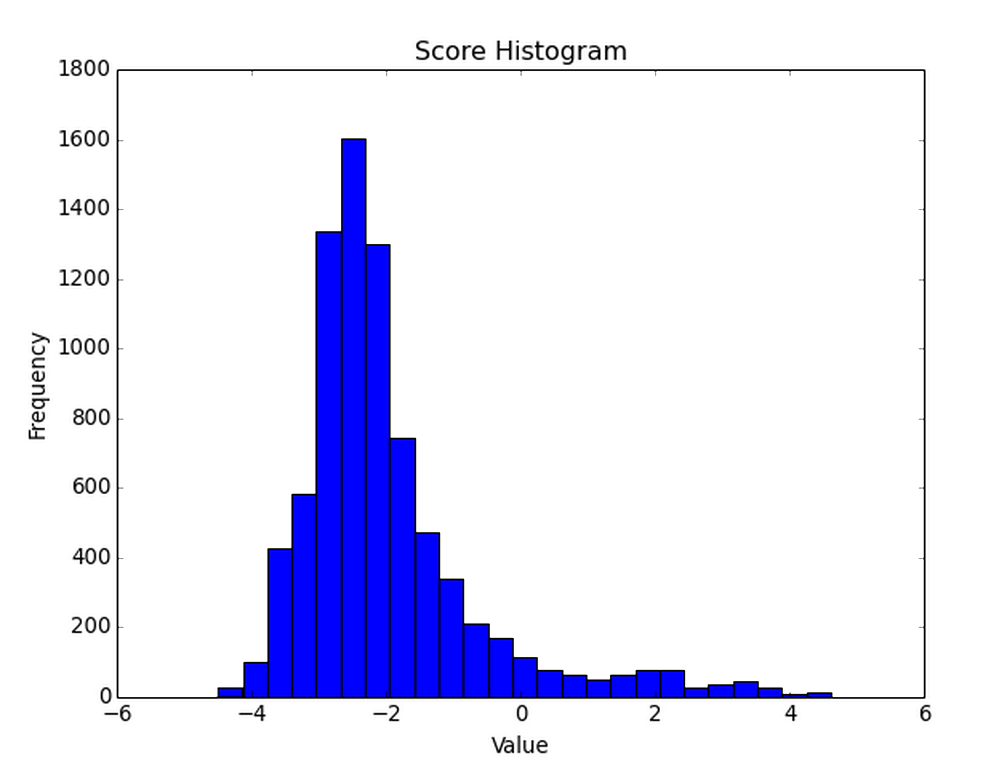
\includegraphics[width=0.6\linewidth]{img/data_hist.png}
  \end{tabular} 
  \caption{Histogram showing the score distribution for the given data} 
  \label{fig:hist_data} 
\end{figure}

% subsection histogram (end)

\subsection{Learning Task} % (fold)
\label{sub:learning_task}
yes
% subsection learning_task (end)

\subsection{Pipeline} % (fold)
\label{sub:pipeline}

% subsection pipeline (end)

\subsection{Evaluation} % (fold)
\label{sub:evaluation}

% subsection evaluation (end)
% section problem_formulation (end)

\section{Preprocessing} % (fold)
\label{sec:preprocessing}
%!TEX root = ../report_nips.tex
\subsection{pp1} % (fold)
\label{sub:pp1}

Lorem ipsum dolor sit amet, consectetur adipisicing elit, sed do eiusmod
tempor incididunt ut labore et dolore magna aliqua. Ut enim ad minim veniam,
quis nostrud exercitation ullamco laboris nisi ut aliquip ex ea commodo
consequat. Duis aute irure dolor in reprehenderit in voluptate velit esse
cillum dolore eu fugiat nulla pariatur. Excepteur sint occaecat cupidatat non
proident, sunt in culpa qui officia deserunt mollit anim id est laborum.

\begin{table}[t]
\caption{Sample table title}
\label{sample-table}
\begin{center}
\begin{tabular}{l | L{4cm} | L{2cm} | L{2cm} | l}
\multicolumn{1}{c}{\bf NAME}  &\multicolumn{1}{c}{\bf DEFINITION} &\multicolumn{2}{c}{\bf EXAMPLE} &\multicolumn{1}{c}{\bf UNIQUE TOKENS}\\
\multicolumn{2}{c}{}  &\multicolumn{1}{c}{\tiny BEFORE} &\multicolumn{1}{c}{\tiny AFTER} &\multicolumn{1}{c}{\bf COUNT}
\\ \hline 

Convert to lowercase &
Converts all characters from a word to lowercase &
PLEASE &
please &
20092 \\ \hline

\multirow{5}{*}{Remove apostrophe} &
\multirow{2}{4cm}{Removes apostrophe and return the original words for most common cases where apostrophe is used as vowel substitution} &
you're &
you are &
\multirow{5}{*}{22718} \\[.6cm]
&&I've & I have & \\[.6cm] \hline


De-elongate words &
Convert elongated words to normal version (works in combination with automated grammar corrector &
pleeeeeeese &
pleease (please – after grammar corrector) &
22640 \\ \hline


\multirow{9}{*}{Remove stop words} &
\multirow{3}{4cm}{There does not exist a single definition of stop words. For our task stop words are words which do not have any sentimental load. We used the stop word list from nltk corpus except words “no” and “not”
under} &
under & &
\multirow{9}{*}{22640}\\[.4cm]
&&before&&\\[.4cm]
&&very&&\\[.4cm]
&&to&&\\[.4cm] \hline



\end{tabular}
\end{center}
\end{table}


% subsection pp1 (end)

\subsection{pp2} % (fold)
\label{sub:pp2}

% subsection pp2 (end)
% section preprocessing (end)

\section{Features} % (fold)
\label{sec:features}
%!TEX root = ../report.tex
\subsection{n-Grams} % (fold)
\label{sub:n_grams}

% subsection n_grams (end)

\subsection{Part of Speec (POS) Tagging} % (fold)
\label{sub:part_of_speec_}

One of the most fundamental parts of the linguistic pipeline is the part-of-speech (POS) tagging, a basic form of syntactic analysis which has countless applications in Natural Language Processing (NLP). We studied some of the best POS tagging tools \& settled on using Tweet NLP, a twitter specific POS tagger. We’ve used part-of-speech tagging as a feature for our task wherein every word/token in a given tweet is tagged based on its part-of-speech, some of which are twitter specific.

For our task, we selected 15 of the most common tags in linguistics (including the twitter specific tags). we made a count of the number of tagged tokens (with a confidence score > 0.9) in a tweet \& then used that as a feature.[rough work]

% subsection part_of_speec_ (end)

\subsection{Sentiment} % (fold)
\label{sub:sentiment}

We used \textit{SentiWordNet} to add features specifically related to the sentiment of the tweets. This is dictionary, designed for opinion mining, where each of the over 100,000 words is assigned a positive and negative sentiment score. For a given tweet, we calculate a positive sum feature: $p_{sum} = \sum_{i}^n p_i$ , where piis the positive sentiment score from SentiWordNet for the ith word in a tweet with n words. We similarly calculate a negative sum feature. If a word is not found in the dictionary, then it does not contribute to either of the two sentiment features. These two features are added to the bag of words feature vector as a real number. It is possible that different preprocessing steps could affect the sentiment score of a tweet by modifying said tweet (such as by stemming); future experimentation is required to determine the effects of different combinations of preprocessing on sentiment score.

% subsection sentiment (end)

\subsection{Irony} % (fold)
\label{sub:irony}

To account for possible irony in the tweets we implement two features based on the work of Reyes et. al [year]. The features are created to detect the so-called \textit{counter-factuality} and \textit{temporal compression} of a tweet. Reyes et. al. determined that ironic tweets were more likely to have a high level of these two measures.

\paragraph{Counter-factuality:} % (fold)
\label{par:counter_factuality_}
The first measure, counter-factuality, is focused on ``discursive terms that hint at opposition or contradiction in a text, such as about, nevertheless, nonetheless, and yet.'' (Citation). The full list of counter-factual words includes 41 entrees; there are a total of 4187 occurrences of these words in the data set, and 3123 tweets contain at least one counter-factual word.
% paragraph counter_factuality_ (end)

\paragraph{Temporal Compression:} % (fold)
\label{par:temporal_compression_}
The second measure of tweet irony that we considered is temporal compression, which focuses on words related to an opposition in time, thus indicating an abrupt change in narrative. (citation) The list of temporal compression words contains 13 words such as suddenly, abruptly, and now. There are only 170 instances of a temporal compression word in the dataset, with only 103 tweets even containing a single instance.
% paragraph temporal_compression_ (end)

\paragraph{Feature Creation:} % (fold)
\label{par:feature_creation_}
For each measure, we create a real-numbered feature based on the ratio of how many words in a given tweet possess the characteristic we are analyzing. That is, we have two ratio features $r_t = \frac{n_t}{n}$, where $t \in \left \{\ex{counterFactuality}, \ex{temporalCompression}\right \}$, $n_t$ is the number of words in a given tweet that fit into category $t$, and $n$ is the total number of words in the tweet.
% paragraph feature_creation_ (end)

% subsection irony (end)
% section features (end)

\newpage
\section{Experiments / Results} % (fold)
\label{sec:experiments_results}
%!TEX root = ../report.tex
\subsection{Experiment 1} % (fold)
\label{sub:experiment_1}

% subsection experiment_1 (end)

\subsection{Experiment 2} % (fold)
\label{sub:experiment_2}

% subsection experiment_2 (end)
% section experiments_results (end)

\section{Conclusion} % (fold)
\label{sec:conclusion}
%!TEX root = ../report.tex
% section conclusion (end)

% \section{Submission of papers to NIPS 2013}

% NIPS requires electronic submissions.  The electronic submission site is  
% \begin{center}
%    \url{http://papers.nips.cc}
% \end{center}

% Please read carefully the
% instructions below, and follow them faithfully.
% \subsection{Style}

% Papers to be submitted to NIPS 2013 must be prepared according to the
% instructions presented here. Papers may be only up to eight pages long,
% including figures. Since 2009 an additional ninth page \textit{containing only
% cited references} is allowed. Papers that exceed nine pages will not be
% reviewed, or in any other way considered for presentation at the conference.
% %This is a strict upper bound. 

% Please note that this year we have introduced automatic line number generation
% into the style file (for \LaTeXe and Word versions). This is to help reviewers
% refer to specific lines of the paper when they make their comments. Please do
% NOT refer to these line numbers in your paper as they will be removed from the
% style file for the final version of accepted papers.

% The margins in 2013 are the same as since 2007, which allow for $\approx 15\%$
% more words in the paper compared to earlier years. We are also again using 
% double-blind reviewing. Both of these require the use of new style files.

% Authors are required to use the NIPS \LaTeX{} style files obtainable at the
% NIPS website as indicated below. Please make sure you use the current files and
% not previous versions. Tweaking the style files may be grounds for rejection.

% %% \subsection{Double-blind reviewing}

% %% This year we are doing double-blind reviewing: the reviewers will not know 
% %% who the authors of the paper are. For submission, the NIPS style file will 
% %% automatically anonymize the author list at the beginning of the paper.

% %% Please write your paper in such a way to preserve anonymity. Refer to
% %% previous work by the author(s) in the third person, rather than first
% %% person. Do not provide Web links to supporting material at an identifiable
% %% web site.

% %%\subsection{Electronic submission}
% %%
% %% \textbf{THE SUBMISSION DEADLINE IS MAY 31st, 2013. SUBMISSIONS MUST BE LOGGED BY
% %% 23:00, MAY 31st, 2013, UNIVERSAL TIME}

% %% You must enter your submission in the electronic submission form available at
% %% the NIPS website listed above. You will be asked to enter paper title, name of
% %% all authors, keyword(s), and data about the contact
% %% author (name, full address, telephone, fax, and email). You will need to
% %% upload an electronic (postscript or pdf) version of your paper.

% %% You can upload more than one version of your paper, until the
% %% submission deadline. We strongly recommended uploading your paper in
% %% advance of the deadline, so you can avoid last-minute server congestion.
% %%
% %% Note that your submission is only valid if you get an e-mail
% %% confirmation from the server. If you do not get such an e-mail, please
% %% try uploading again. 


% \subsection{Retrieval of style files}

% The style files for NIPS and other conference information are available on the World Wide Web at
% \begin{center}
%    \url{http://www.nips.cc/}
% \end{center}
% The file \verb+nips2013.pdf+ contains these 
% instructions and illustrates the
% various formatting requirements your NIPS paper must satisfy. \LaTeX{}
% users can choose between two style files:
% \verb+nips11submit_09.sty+ (to be used with \LaTeX{} version 2.09) and
% \verb+nips11submit_e.sty+ (to be used with \LaTeX{}2e). The file
% \verb+nips2013.tex+ may be used as a ``shell'' for writing your paper. All you
% have to do is replace the author, title, abstract, and text of the paper with
% your own. The file
% \verb+nips2013.rtf+ is provided as a shell for MS Word users.

% The formatting instructions contained in these style files are summarized in
% sections \ref{gen_inst}, \ref{headings}, and \ref{others} below.

% %% \subsection{Keywords for paper submission}
% %% Your NIPS paper can be submitted with any of the following keywords (more than one keyword is possible for each paper):

% %% \begin{verbatim}
% %% Bioinformatics
% %% Biological Vision
% %% Brain Imaging and Brain Computer Interfacing
% %% Clustering
% %% Cognitive Science
% %% Control and Reinforcement Learning
% %% Dimensionality Reduction and Manifolds
% %% Feature Selection
% %% Gaussian Processes
% %% Graphical Models
% %% Hardware Technologies
% %% Kernels
% %% Learning Theory
% %% Machine Vision
% %% Margins and Boosting
% %% Neural Networks
% %% Neuroscience
% %% Other Algorithms and Architectures
% %% Other Applications
% %% Semi-supervised Learning
% %% Speech and Signal Processing
% %% Text and Language Applications

% %% \end{verbatim}

% \section{General formatting instructions}
% \label{gen_inst}

% The text must be confined within a rectangle 5.5~inches (33~picas) wide and
% 9~inches (54~picas) long. The left margin is 1.5~inch (9~picas).
% Use 10~point type with a vertical spacing of 11~points. Times New Roman is the
% preferred typeface throughout. Paragraphs are separated by 1/2~line space,
% with no indentation.

% Paper title is 17~point, initial caps/lower case, bold, centered between
% 2~horizontal rules. Top rule is 4~points thick and bottom rule is 1~point
% thick. Allow 1/4~inch space above and below title to rules. All pages should
% start at 1~inch (6~picas) from the top of the page.

% %The version of the paper submitted for review should have ``Anonymous Author(s)'' as the author of the paper.

% For the final version, authors' names are
% set in boldface, and each name is centered above the corresponding
% address. The lead author's name is to be listed first (left-most), and
% the co-authors' names (if different address) are set to follow. If
% there is only one co-author, list both author and co-author side by side.

% Please pay special attention to the instructions in section \ref{others}
% regarding figures, tables, acknowledgments, and references.

% \section{Headings: first level}
% \label{headings}

% First level headings are lower case (except for first word and proper nouns),
% flush left, bold and in point size 12. One line space before the first level
% heading and 1/2~line space after the first level heading.

% \subsection{Headings: second level}

% Second level headings are lower case (except for first word and proper nouns),
% flush left, bold and in point size 10. One line space before the second level
% heading and 1/2~line space after the second level heading.

% \subsubsection{Headings: third level}

% Third level headings are lower case (except for first word and proper nouns),
% flush left, bold and in point size 10. One line space before the third level
% heading and 1/2~line space after the third level heading.

% \section{Citations, figures, tables, references}
% \label{others}

% These instructions apply to everyone, regardless of the formatter being used.

% \subsection{Citations within the text}

% Citations within the text should be numbered consecutively. The corresponding
% number is to appear enclosed in square brackets, such as [1] or [2]-[5]. The
% corresponding references are to be listed in the same order at the end of the
% paper, in the \textbf{References} section. (Note: the standard
% \textsc{Bib\TeX} style \texttt{unsrt} produces this.) As to the format of the
% references themselves, any style is acceptable as long as it is used
% consistently.

% As submission is double blind, refer to your own published work in the 
% third person. That is, use ``In the previous work of Jones et al.\ [4]'',
% not ``In our previous work [4]''. If you cite your other papers that
% are not widely available (e.g.\ a journal paper under review), use
% anonymous author names in the citation, e.g.\ an author of the
% form ``A.\ Anonymous''. 


% \subsection{Footnotes}

% Indicate footnotes with a number\footnote{Sample of the first footnote} in the
% text. Place the footnotes at the bottom of the page on which they appear.
% Precede the footnote with a horizontal rule of 2~inches
% (12~picas).\footnote{Sample of the second footnote}

% \subsection{Figures}

% All artwork must be neat, clean, and legible. Lines should be dark
% enough for purposes of reproduction; art work should not be
% hand-drawn. The figure number and caption always appear after the
% figure. Place one line space before the figure caption, and one line
% space after the figure. The figure caption is lower case (except for
% first word and proper nouns); figures are numbered consecutively.

% Make sure the figure caption does not get separated from the figure.
% Leave sufficient space to avoid splitting the figure and figure caption.

% You may use color figures. 
% However, it is best for the
% figure captions and the paper body to make sense if the paper is printed
% either in black/white or in color.
% \begin{figure}[h]
% \begin{center}
% %\framebox[4.0in]{$\;$}
% \fbox{\rule[-.5cm]{0cm}{4cm} \rule[-.5cm]{4cm}{0cm}}
% \end{center}
% \caption{Sample figure caption.}
% \end{figure}

% \subsection{Tables}

% All tables must be centered, neat, clean and legible. Do not use hand-drawn
% tables. The table number and title always appear before the table. See
% Table~\ref{sample-table}.

% Place one line space before the table title, one line space after the table
% title, and one line space after the table. The table title must be lower case
% (except for first word and proper nouns); tables are numbered consecutively.

% \begin{table}[t]
% \caption{Sample table title}
% \label{sample-table}
% \begin{center}
% \begin{tabular}{ll}
% \multicolumn{1}{c}{\bf PART}  &\multicolumn{1}{c}{\bf DESCRIPTION}
% \\ \hline \\
% Dendrite         &Input terminal \\
% Axon             &Output terminal \\
% Soma             &Cell body (contains cell nucleus) \\
% \end{tabular}
% \end{center}
% \end{table}

% \section{Final instructions}
% Do not change any aspects of the formatting parameters in the style files.
% In particular, do not modify the width or length of the rectangle the text
% should fit into, and do not change font sizes (except perhaps in the
% \textbf{References} section; see below). Please note that pages should be
% numbered.

% \section{Preparing PostScript or PDF files}

% Please prepare PostScript or PDF files with paper size ``US Letter'', and
% not, for example, ``A4''. The -t
% letter option on dvips will produce US Letter files.

% Fonts were the main cause of problems in the past years. Your PDF file must
% only contain Type 1 or Embedded TrueType fonts. Here are a few instructions
% to achieve this.

% \begin{itemize}

% \item You can check which fonts a PDF files uses.  In Acrobat Reader,
% select the menu Files$>$Document Properties$>$Fonts and select Show All Fonts. You can
% also use the program \verb+pdffonts+ which comes with \verb+xpdf+ and is
% available out-of-the-box on most Linux machines.

% \item The IEEE has recommendations for generating PDF files whose fonts
% are also acceptable for NIPS. Please see
% \url{http://www.emfield.org/icuwb2010/downloads/IEEE-PDF-SpecV32.pdf}

% \item LaTeX users:

% \begin{itemize}

% \item Consider directly generating PDF files using \verb+pdflatex+
% (especially if you are a MiKTeX user). 
% PDF figures must be substituted for EPS figures, however.

% \item Otherwise, please generate your PostScript and PDF files with the following commands:
% \begin{verbatim} 
% dvips mypaper.dvi -t letter -Ppdf -G0 -o mypaper.ps
% ps2pdf mypaper.ps mypaper.pdf
% \end{verbatim}

% Check that the PDF files only contains Type 1 fonts. 
% %For the final version, please send us both the Postscript file and
% %the PDF file. 

% \item xfig "patterned" shapes are implemented with 
% bitmap fonts.  Use "solid" shapes instead. 
% \item The \verb+\bbold+ package almost always uses bitmap
% fonts.  You can try the equivalent AMS Fonts with command
% \begin{verbatim}
% \usepackage[psamsfonts]{amssymb}
% \end{verbatim}
%  or use the following workaround for reals, natural and complex: 
% \begin{verbatim}
% \newcommand{\RR}{I\!\!R} %real numbers
% \newcommand{\Nat}{I\!\!N} %natural numbers 
% \newcommand{\CC}{I\!\!\!\!C} %complex numbers
% \end{verbatim}

% \item Sometimes the problematic fonts are used in figures
% included in LaTeX files. The ghostscript program \verb+eps2eps+ is the simplest
% way to clean such figures. For black and white figures, slightly better
% results can be achieved with program \verb+potrace+.
% \end{itemize}
% \item MSWord and Windows users (via PDF file):
% \begin{itemize}
% \item Install the Microsoft Save as PDF Office 2007 Add-in from
% \url{http://www.microsoft.com/downloads/details.aspx?displaylang=en\&familyid=4d951911-3e7e-4ae6-b059-a2e79ed87041}
% \item Select ``Save or Publish to PDF'' from the Office or File menu
% \end{itemize}
% \item MSWord and Mac OS X users (via PDF file):
% \begin{itemize}
% \item From the print menu, click the PDF drop-down box, and select ``Save
% as PDF...''
% \end{itemize}
% \item MSWord and Windows users (via PS file):
% \begin{itemize}
% \item To create a new printer
% on your computer, install the AdobePS printer driver and the Adobe Distiller PPD file from
% \url{http://www.adobe.com/support/downloads/detail.jsp?ftpID=204} {\it Note:} You must reboot your PC after installing the
% AdobePS driver for it to take effect.
% \item To produce the ps file, select ``Print'' from the MS app, choose
% the installed AdobePS printer, click on ``Properties'', click on ``Advanced.''
% \item Set ``TrueType Font'' to be ``Download as Softfont''
% \item Open the ``PostScript Options'' folder
% \item Select ``PostScript Output Option'' to be ``Optimize for Portability''
% \item Select ``TrueType Font Download Option'' to be ``Outline''
% \item Select ``Send PostScript Error Handler'' to be ``No''
% \item Click ``OK'' three times, print your file.
% \item Now, use Adobe Acrobat Distiller or ps2pdf to create a PDF file from
% the PS file. In Acrobat, check the option ``Embed all fonts'' if
% applicable.
% \end{itemize}

% \end{itemize}
% If your file contains Type 3 fonts or non embedded TrueType fonts, we will
% ask you to fix it. 

% \subsection{Margins in LaTeX}
 
% Most of the margin problems come from figures positioned by hand using
% \verb+\special+ or other commands. We suggest using the command
% \verb+\includegraphics+
% from the graphicx package. Always specify the figure width as a multiple of
% the line width as in the example below using .eps graphics
% \begin{verbatim}
%    \usepackage[dvips]{graphicx} ... 
%    \includegraphics[width=0.8\linewidth]{myfile.eps} 
% \end{verbatim}
% or % Apr 2009 addition
% \begin{verbatim}
%    \usepackage[pdftex]{graphicx} ... 
%    \includegraphics[width=0.8\linewidth]{myfile.pdf} 
% \end{verbatim}
% for .pdf graphics. 
% See section 4.4 in the graphics bundle documentation (\url{http://www.ctan.org/tex-archive/macros/latex/required/graphics/grfguide.ps}) 
 
% A number of width problems arise when LaTeX cannot properly hyphenate a
% line. Please give LaTeX hyphenation hints using the \verb+\-+ command.


\subsubsection*{Acknowledgments}

Use unnumbered third level headings for the acknowledgments. All
acknowledgments go at the end of the paper. Do not include 
acknowledgments in the anonymized submission, only in the 
final paper. 

\subsubsection*{References}

References follow the acknowledgments. Use unnumbered third level heading for
the references. Any choice of citation style is acceptable as long as you are
consistent. It is permissible to reduce the font size to `small' (9-point) 
when listing the references. {\bf Remember that this year you can use
a ninth page as long as it contains \emph{only} cited references.}

\small{
[1] Alexander, J.A. \& Mozer, M.C. (1995) Template-based algorithms
for connectionist rule extraction. In G. Tesauro, D. S. Touretzky
and T.K. Leen (eds.), {\it Advances in Neural Information Processing
Systems 7}, pp. 609-616. Cambridge, MA: MIT Press.

[2] Bower, J.M. \& Beeman, D. (1995) {\it The Book of GENESIS: Exploring
Realistic Neural Models with the GEneral NEural SImulation System.}
New York: TELOS/Springer-Verlag.

[3] Hasselmo, M.E., Schnell, E. \& Barkai, E. (1995) Dynamics of learning
and recall at excitatory recurrent synapses and cholinergic modulation
in rat hippocampal region CA3. {\it Journal of Neuroscience}
{\bf 15}(7):5249-5262.
}

\end{document}